% THIS IS SIGPROC-SP.TEX - VERSION 3.1
% WORKS WITH V3.2SP OF ACM_PROC_ARTICLE-SP.CLS
% APRIL 2009
%
% It is an example file showing how to use the 'acm_proc_article-sp.cls' V3.2SP
% LaTeX2e document class file for Conference Proceedings submissions.
% ----------------------------------------------------------------------------------------------------------------
% This .tex file (and associated .cls V3.2SP) *DOES NOT* produce:
%       1) The Permission Statement
%       2) The Conference (location) Info information
%       3) The Copyright Line with ACM data
%       4) Page numbering
% ---------------------------------------------------------------------------------------------------------------
% It is an example which *does* use the .bib file (from which the .bbl file
% is produced).
% REMEMBER HOWEVER: After having produced the .bbl file,
% and prior to final submission,
% you need to 'insert'  your .bbl file into your source .tex file so as to provide
% ONE 'self-contained' source file.
%
% Questions regarding SIGS should be sent to
% Adrienne Griscti ---> griscti@acm.org
%
% Questions/suggestions regarding the guidelines, .tex and .cls files, etc. to
% Gerald Murray ---> murray@hq.acm.org
%
% For tracking purposes - this is V3.1SP - APRIL 2009

\documentclass{acm_proc_article-sp}

\usepackage{caption}
\usepackage{soul}
\usepackage{color}
\usepackage{url}
\usepackage{hyperref}
\usepackage{subfig}
\usepackage{graphicx}

\begin{document}
\title{Using Markov Chains to Identify Sequences as CpG or non CpG Islands}
\subtitle{Assignment 2}
%
% You need the command \numberofauthors to handle the 'placement
% and alignment' of the authors beneath the title.
%
% For aesthetic reasons, we recommend 'three authors at a time'
% i.e. three 'name/affiliation blocks' be placed beneath the title.
%
% NOTE: You are NOT restricted in how many 'rows' of
% "name/affiliations" may appear. We just ask that you restrict
% the number of 'columns' to three.
%
% Because of the available 'opening page real-estate'
% we ask you to refrain from putting more than six authors
% (two rows with three columns) beneath the article title.
% More than six makes the first-page appear very cluttered indeed.
%
% Use the \alignauthor commands to handle the names
% and affiliations for an 'aesthetic maximum' of six authors.
% Add names, affiliations, addresses for
% the seventh etc. author(s) as the argument for the
% \additionalauthors command.
% These 'additional authors' will be output/set for you
% without further effort on your part as the last section in
% the body of your article BEFORE References or any Appendices.

%\numberofauthors{3} %  in this sample file, there are a *total*
% of EIGHT authors. SIX appear on the 'first-page' (for formatting
% reasons) and the remaining two appear in the \additionalauthors section.
%
\numberofauthors{1}
\author{
	\alignauthor Caitlin Ross\\
	\affaddr{Computer Science Department, Rensselaer Polytechnic Institute} \\
	\email{rossc3@rpi.edu}
}
% There's nothing stopping you putting the seventh, eighth, etc.
% author on the opening page (as the 'third row') but we ask,
% for aesthetic reasons that you place these 'additional authors'
% in the \additional authors block, viz.

\date{30 July 1999}
% Just remember to make sure that the TOTAL number of authors
% is the number that will appear on the first page PLUS the
% number that will appear in the \additionalauthors section.

\maketitle

\begin{abstract}
This work looks at the use of Markov chains to model CpG island regions.  Previously identified CpG islands from human chromosome 12 and random non-CpG island sequences from the same chromosome are used to determine the transition matrices for the Markov model.  The model is tested using test sets collected from the same data sets.  To test the model, each test sequence has its log odds ratio calculated.  Based on a histogram plot of the log odds ratios, the model appears to model the sequences as expected, with the CpG test sequences having a positive log odds ratio, while the non-CpG test sequences tend to have negative log odds ratios.  Finally the log odds ratios of 10 unknown sequences are calculated in order to determine whether it is likely for the sequence to be a CpG island or not.  
\end{abstract}


\section{Problem Statement}
The problem studied here is to use Markov chains to model CpG island regions.  To do this, we need a set of previously identified CpG islands and a full chromosome sequence.  The CpG sequences will form a positive training set for our model, while randomly chosen sequences from the chromosome sequence will form the negative training set for the model.  The two training sets are used to find their respective group's transition matrix.  At this point the positive and negative sets' transition matrices can be used to calculate the log odds ratio of an unknown sequence in order to determine whether this sequence is likely to be a CpG island or not.  

\section{Methods}
This section first discusses the relevant mathematics to this work, followed by a description of the program developed.
\subsection{Relevant Mathematics}
\label{sec:math}
A Markov chain consists of states that undergo transitions from one state to another.  Each transition is assigned some probability, which depends only on the current state and not any previous states.  In this model, there are 16 transitions for each pair of bases.  From textbook `Biological Sequence Analysis' by Durbin et al., the transition probability is defined as
 \begin{equation}a_{st} = P(x_{i} = t | x_{i-1} = s)\end{equation}
(i.e. $a_{st}$ is the probability that t follows s in the sequence).  

The probability of a given sequence x, is 
\begin{equation} P(x) = P(x_{1}) \prod\limits_{i=2}^L a_{x_{i-1},x_{i}} \end{equation}
where L is the length of the sequence and $x_{i}$ are letters in the sequence.

To find the transition probabilities for the positive training model, the following equation was used:
\begin{equation} a_{st}^+ = \frac{c_{st}^+}{\sum_{t'}c_{st'}^+}\end{equation}
where $c_{st}^+$ is the number of times that t follows s in the sequence and $t'$ represents any letter in the alphabet used.  Equation (3) is also used similarly to find $a_{st}^-$ for the negative training set.

To compute the log odds ratio of a given sequence once the transition matrices are found, the following equation is used:
\begin{equation} \sum\limits_{i=2}^L \log{\frac{a^+_{x_{i-1},x_{i}}}{a^-_{x_{i-1},x_{i}}}} \end{equation}
where $x_{i} \in {A,C,T,G}$.

\subsection{Program}
The program uses the files \texttt{CpG} and \texttt{chr12.fa}.  The file \texttt{CpG} was downloaded from \hyperref[http://genome.ucsc.edu/cgi-bin/hgTables?hgsid=444312915_EcUDmaoda0cHkB6XzADvJ9eK7PZM]{http://genome.ucsc.edu} and contains 1211 FASTA sequences.  These sequences are from CpG islands found in the human genome on chromosome 12 using the December 2013 assembly.  `chr12.fa' is a FASTA file downloaded from \hyperref[http://hgdownload.cse.ucsc.edu/goldenPath/hg38/chromosomes/]{http://hgdownload.cse.ucsc.edu} that contains the full DNA sequence for human chromosome 12. These two files are used to build the Markov chain model and then to test that the model is correct.  The program also uses the file \texttt{test\_sequences.fasta}, downloaded from the course website.  This file is another FASTA file, that contains 10 sequences from different mammalian genomes.  The Markov model is used to identify the sequences in this file as likely or unlikely to be CpG islands.

The program uses Biopython to read the FASTA files.  The function \texttt{pos\_samp()} reads the \texttt{CpG} file to get the sequences. It then randomly chooses 200 sequences to return as the positive training set, and the other 1011 sequences as the positive test set.

The program then creates the negative training and test sets from the chromosome 12 DNA sequence from \texttt{chr12.fa}.  The function \texttt{random\_seq()} takes in the chromosome DNA sequence, and the length of the sequence the function should return. Since the CpG sequences are a small portion of the chromosome 12 sequence, choosing sequences from random in the chromosome will be likely to return non-CpG sequences.  For every CpG sequence in the positive sets, the length is used to choose the size of the sequences in the negative sets. 

The program then uses the positive and negative training sets to find the transition matrix for each set for the Markov model using equation (3), as explained in Section \ref{sec:math}.  The program uses the function \texttt{calc\_trans\_matrix()}, which takes in one of the training sets to calculate its transition matrix.  

Now that both transition matrices are found, they can be used to find the log odds ratio in equation (4) of an unknown sequence.  First we use the positive and negative training sets to test the correctness of the transition matrices.  Each sequence in these sets is passed to the function \texttt{calc\_log\_odds\_ratio()}, which calculates the log odds ratio of the sequence and normalizes the value by dividing by the length of the sequence.  Then a histogram of the counts of the log odds ratio is plotted.

After this, the program reads in the sequences contained in the \texttt{test\_sequences.fasta} file.  The normalized log odds ratio of these sequences are found.  If the normalized log odds ratio is positive, it is considered to most likely be a CpG island, otherwise it's considered unlikely to be a CpG island.  

\section{Results}
Tables \ref{posmat} and \ref{negmat} show the transition matrices for the positive and negative sets, respectively.  In the positive set's matrix, the C and G nucleotides columns show the highest probabilities.  Since this matrix is created from the set of CpG island sequences, it is expected that C and G are more likely to follow another nucleotide than A and T.  This trend doesn't hold in the negative training set's transition matrix.  One thing to note is that the probability of a G to follow a C is only approximately 5\%.  So CpGs are rarely found in the random sequences from Chromosome 12.  

Figure 1 shows the histogram of the log odds ratios calculated from the positive and negative tests sets.  Based on the histogram, the Markov model appears to be correct as the CpG sequences mostly have positive log odds ratios, while most of the ratios for the random chromosome 12 sequences are negative.  


Table \ref{logodds} shows the log odds ratios for the 10 sequences contained in \texttt{test\_sequences.fasta}.  Sequences 0, 2, 3, 4, 8, and 9 appear to be CpG islands, based on their log odds ratios.  Sequences 1 and 7 appear to be non-CpG islands based on their log odds ratio as well.  Sequences 5 and 6 have negative log odds ratios as well, however their ratios are close to 0, so it's not as certain that they are non-CpG islands.  

\begin{table}
\centering
\caption{Positive Training Set Transition Matrix}
\label{posmat}
\begin{tabular}{|c|c|c|c|c|} \hline
 +&A&C&G&T\\ \hline
A  &0.19704 &0.26645 &0.41745 &0.11905 \\ \hline
C  &0.15636  &0.36629  &0.28588  &0.19147 \\ \hline
G  &0.16457  &0.35469  &0.35954  &0.12119 \\ \hline
T  &0.08902  &0.36991  &0.34713  &0.19394\\ 
\hline\end{tabular}
\vspace{1.8em}
\caption{Negative Training Set Transition Matrix}
\label{negmat}
\begin{tabular}{|c|c|c|c|c|} \hline
- &A&C&G&T\\ \hline
A  &0.32785  &0.16925  &0.23915  &0.26374 \\ \hline
C  &0.35308  &0.25461  &0.05246  &0.33985 \\ \hline
G  &0.28183  &0.21274  &0.25446  &0.25096 \\ \hline
T  &0.21691  &0.19940  &0.24718  &0.33652 \\
\hline\end{tabular}
\end{table}

\begin{table}
\centering
\caption{Negative Training Set Transition Matrix}
\label{logodds}
\begin{tabular}{|c|c|} \hline
Sequence ID & Log Odds Ratio\\ \hline
0 & 0.30956 \\ \hline
1 & -0.13199 \\ \hline
2 & 0.23125 \\ \hline
3 & 0.14662 \\ \hline
4 & 0.17286 \\ \hline
5 & -0.00964 \\ \hline
6 & -0.06452 \\ \hline
7 & -0.39547 \\ \hline
8 & 0.36713 \\ \hline
9 & 0.15661 \\ 
\hline\end{tabular}
\end{table}

\begin{figure}[!b]
	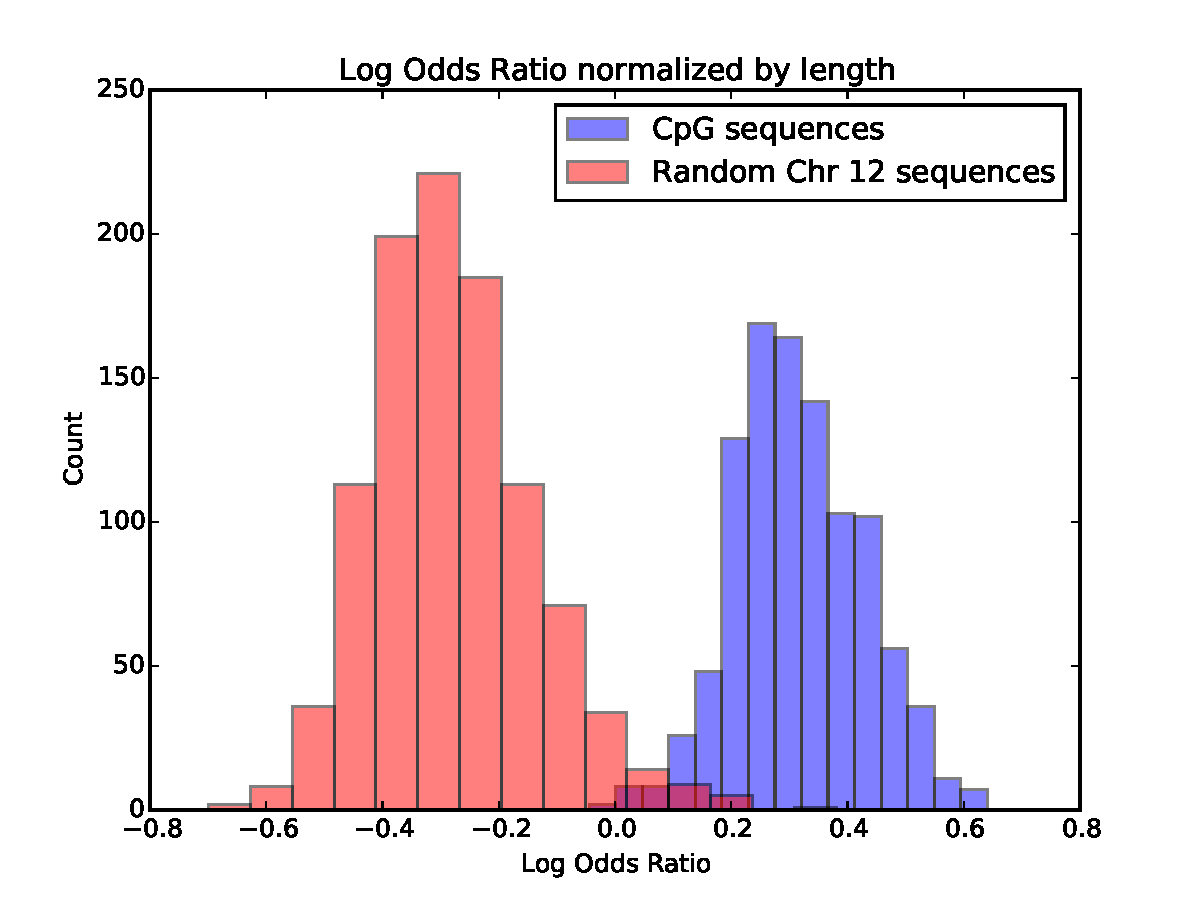
\includegraphics[trim={0 0 2cm 0}, clip,width=3.5in]{histogram.pdf}
	\caption{Histogram of log odds ratios of the positive and negative test sets normalized for the length of the sequences}
	\label{fig:hist}
\end{figure}



%
% The following two commands are all you need in the
% initial runs of your .tex file to
% produce the bibliography for the citations in your paper.
\bibliographystyle{abbrv}
%\bibliography{sigproc}  % sigproc.bib is the name of the Bibliography in this case

% You must have a proper ".bib" file
%  and remember to run:
% latex bibtex latex latex
% to resolve all references
%
% ACM needs 'a single self-contained file'!
%
%APPENDICES are optional
%\balancecolumns

\balancecolumns
% That's all folks!
\end{document}
